\documentclass[aspectratio=169,11pt]{beamer}

\usepackage{fontspec}
\setsansfont{DejaVu Sans}
\setmonofont{DejaVu Sans Mono}
\usepackage[spanish,es-nodecimaldot]{babel}
\usepackage{booktabs}
\usepackage{graphicx}
\usepackage{listings}
\usepackage{xcolor}

\definecolor{azul}{HTML}{264653}
\definecolor{verde}{HTML}{2A9D8F}
\definecolor{arena}{HTML}{E9C46A}
\definecolor{naranja}{HTML}{E76F51}
\definecolor{tinta}{HTML}{263238}
\definecolor{papel}{HTML}{F7F7F4}

\setbeamercolor{normal text}{fg=tinta,bg=white}
\setbeamercolor{structure}{fg=verde}
\setbeamercolor{frametitle}{fg=white,bg=azul}
\setbeamercolor{title}{fg=white}
\setbeamertemplate{navigation symbols}{}
\setbeamertemplate{itemize item}{\color{verde}\small$\blacktriangleright$}
\setbeamertemplate{footline}{%
  \hfill\usebeamerfont{page number in head/foot}%
  \color{azul}\insertframenumber\hspace{0.5cm}\vspace{0.25cm}}

\lstdefinelanguage{R}{
  morekeywords={library,if,else,TRUE,FALSE,function},
  sensitive=true,
  morecomment=[l]{\#},
  morestring=[b]"
}
\lstset{
  language=R,
  basicstyle=\ttfamily\footnotesize,
  keywordstyle=\color{naranja}\bfseries,
  commentstyle=\color{azul!70},
  stringstyle=\color{verde!80!black},
  backgroundcolor=\color{papel},
  frame=single,
  rulecolor=\color{azul!20},
  frameround=tttt,
  breaklines=true,
  showstringspaces=false,
  columns=fullflexible,
  keepspaces=true,
  aboveskip=0.25em,
  belowskip=0.25em,
  literate={á}{{á}}1 {é}{{é}}1 {í}{{í}}1 {ó}{{ó}}1 {ú}{{ú}}1
           {ñ}{{ñ}}1 {±}{{$\pm$}}1
}

\graphicspath{{resultados/infografia_ggplot/}{../resultados/infografia_ggplot/}}
\title{ggplot2 por capas: gráfica de cajas para publicación científica}

\begin{document}

% Lámina 1
\begin{frame}[plain]
  \begin{beamercolorbox}[wd=\paperwidth,ht=\paperheight,dp=0pt]{frametitle}
    \vspace{1.65cm}
    \hspace{1.2cm}\begin{minipage}{0.80\paperwidth}\raggedright
      {\usebeamerfont{title}\fontsize{29}{34}\selectfont\inserttitle\par}
    \end{minipage}
  \end{beamercolorbox}
\end{frame}

% Lámina 2
\begin{frame}[fragile]{La gramática de ggplot2}
\begin{columns}[T,onlytextwidth]
\column{0.39\textwidth}
\begin{lstlisting}[basicstyle=\ttfamily\footnotesize]
ggplot(datos, aes(x, y)) +
  geom_*() +
  scale_*() +
  labs() +
  theme_*()
\end{lstlisting}

\small El signo \texttt{+} agrega una capa sin modificar el dataframe original.

\column{0.58\textwidth}
\small
{\setlength{\tabcolsep}{3pt}\begin{tabular}{@{}lp{5.4cm}@{}}
\toprule
\textbf{Componente} & \textbf{Pregunta que responde}\\
\midrule
\texttt{datos} & ¿Qué dataframe contiene las observaciones?\\
\texttt{aes()} & ¿Qué variable ocupa cada eje o propiedad visual?\\
\texttt{geom\_*()} & ¿Cómo se representan los datos: puntos, cajas o líneas?\\
\texttt{scale\_*()} & ¿Qué orden, colores o transformaciones se utilizan?\\
\texttt{labs()} & ¿Qué nombres y unidades verá el lector?\\
\texttt{theme\_*()} & ¿Cómo se presenta la figura?\\
\bottomrule
\end{tabular}}
\end{columns}
\end{frame}

% Lámina 3
\begin{frame}[fragile]{Paso 1. Datos, ejes y geometría}
\begin{columns}[T,onlytextwidth]
  \column{0.45\textwidth}
\begin{lstlisting}
ggplot(
  datos_limpios,
  aes(
    x = grupo,
    y = pcr_mg_l
  )
) +
  geom_boxplot()
\end{lstlisting}

\small
\texttt{x} contiene los grupos clínicos.\\[0.15cm]
\texttt{y} contiene la proteína C reactiva.\\[0.15cm]
\texttt{geom\_boxplot()} calcula y dibuja las cajas.
  \column{0.53\textwidth}
  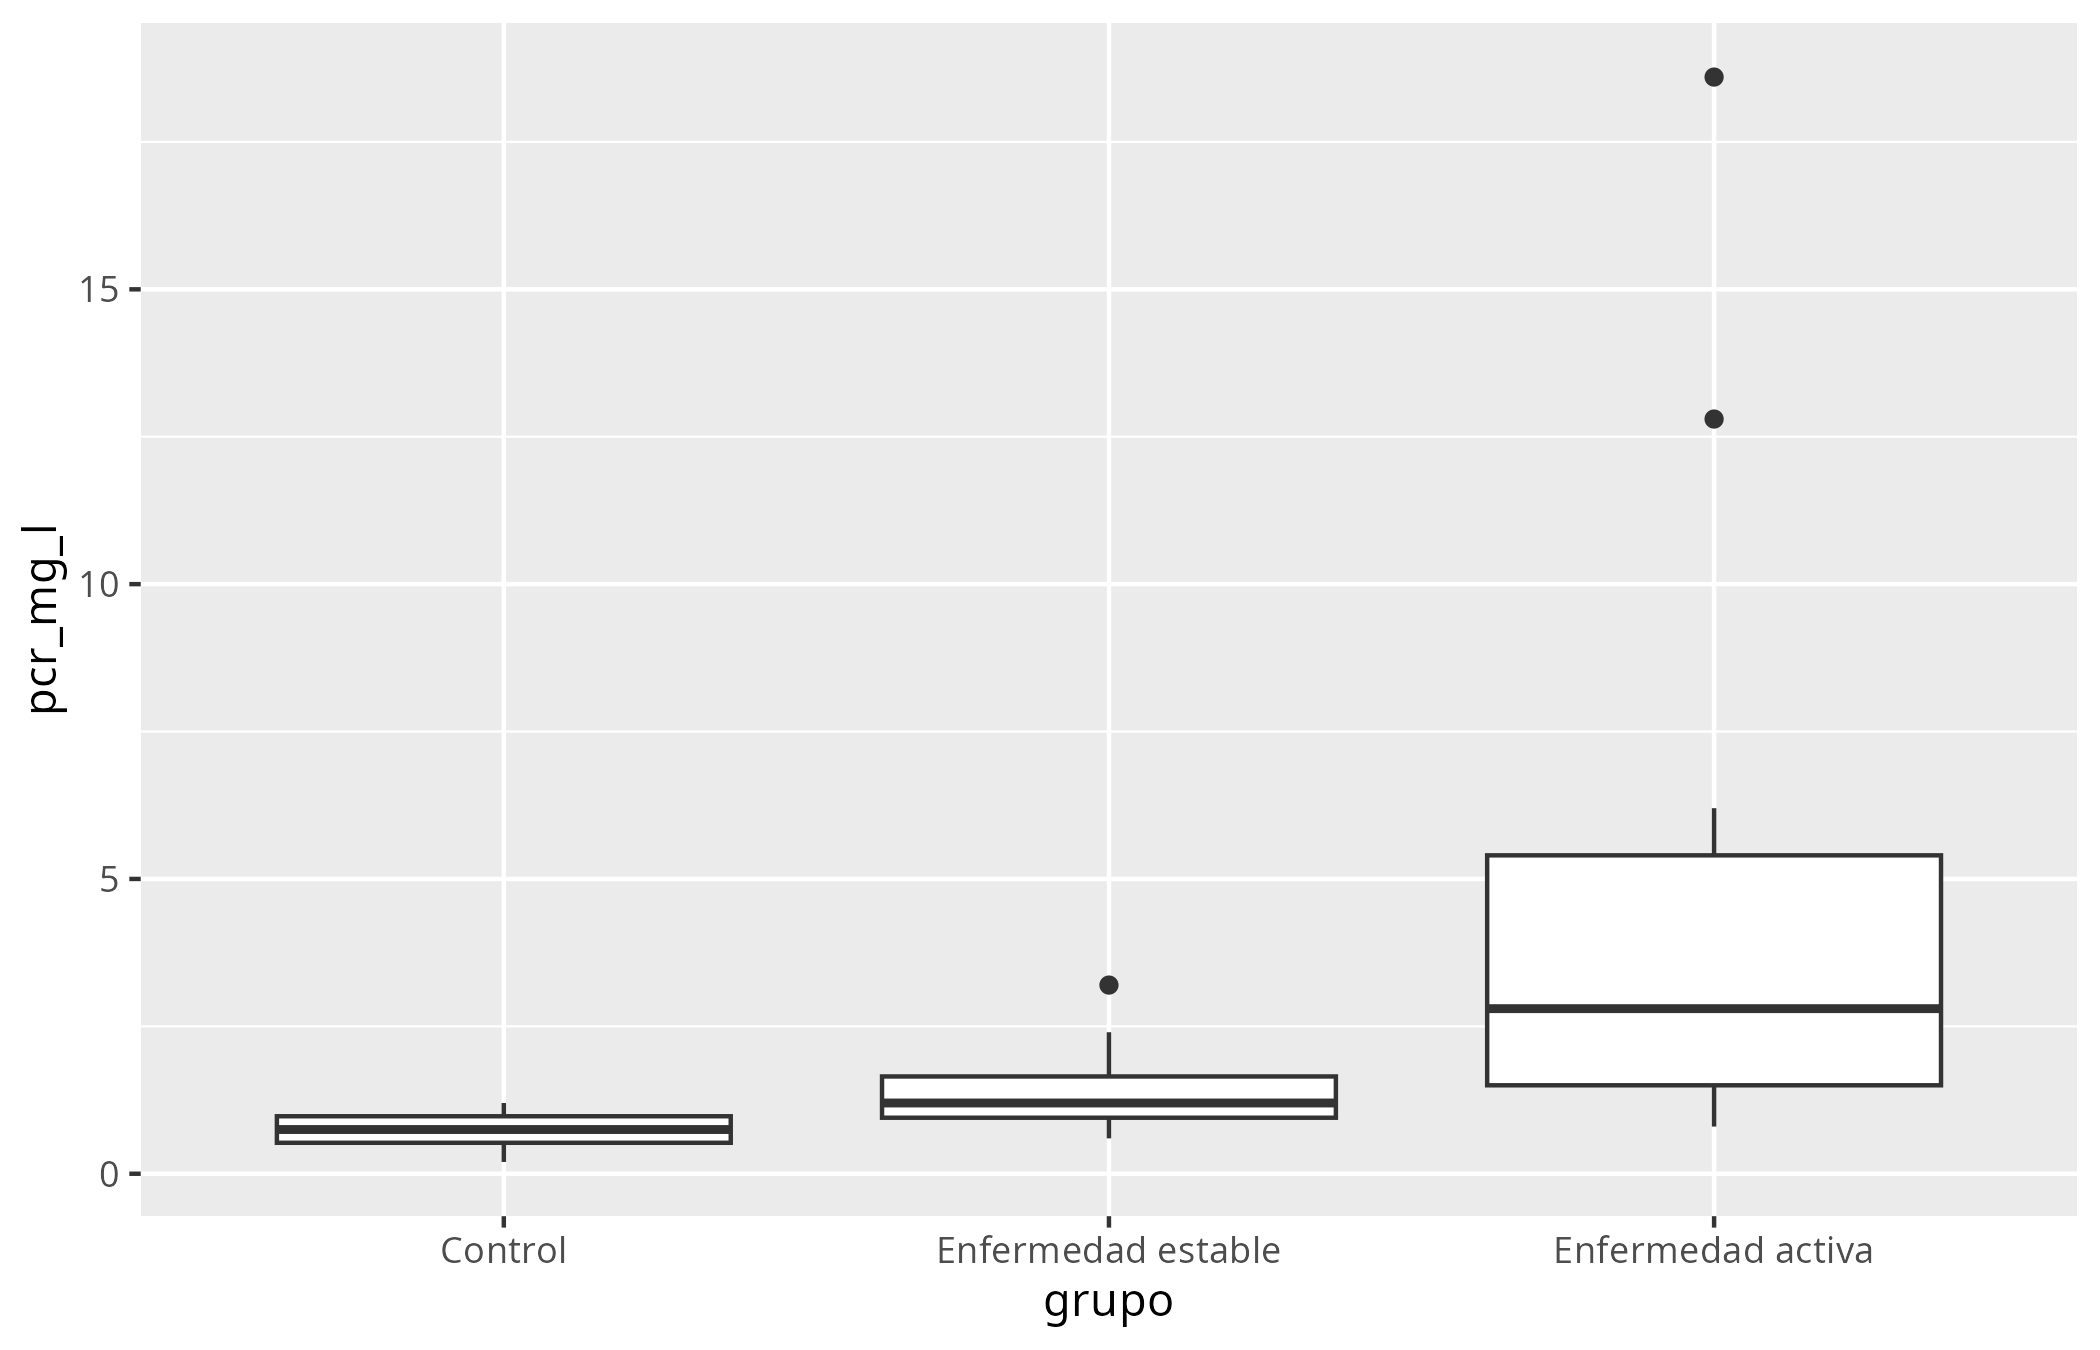
\includegraphics[width=\linewidth]{paso_1_caja.png}
\end{columns}
\end{frame}

% Lámina 4
\begin{frame}[fragile]{Paso 2. Observaciones individuales}
\begin{columns}[T,onlytextwidth]
  \column{0.46\textwidth}
\begin{lstlisting}[basicstyle=\ttfamily\scriptsize]
geom_boxplot(
  outlier.shape = NA
) +
geom_point(
  position = position_jitter(
    width = 0.10,
    seed = 123
  ),
  alpha = 0.75,
  size = 2
)
\end{lstlisting}

\small Cada punto representa un paciente. \texttt{seed} conserva la misma posición al repetir el análisis.
  \column{0.52\textwidth}
  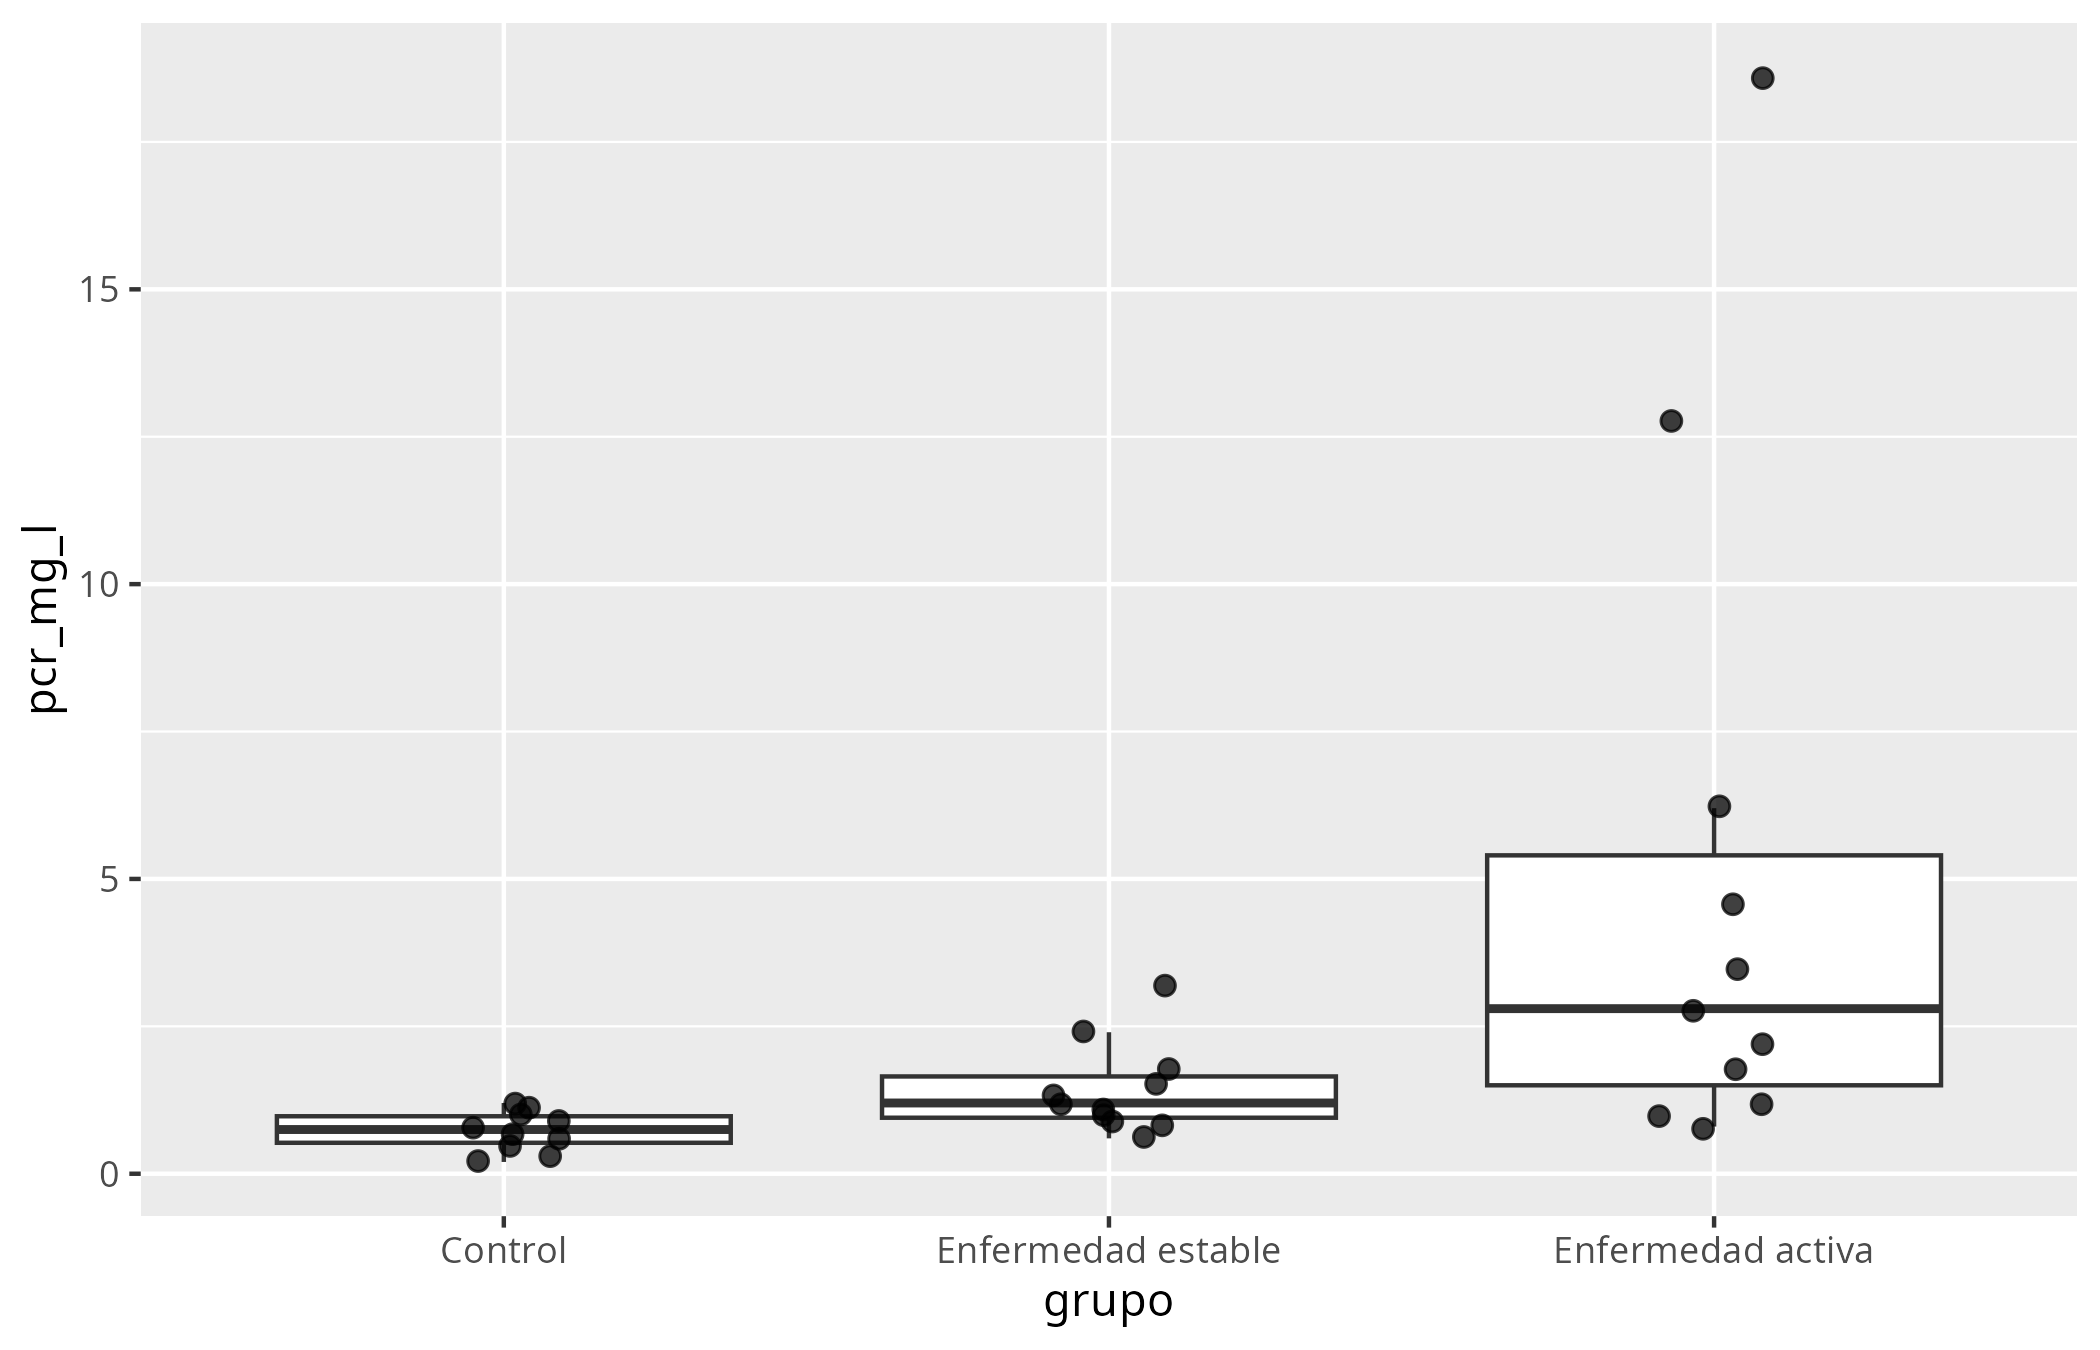
\includegraphics[width=\linewidth]{paso_2_puntos.png}
\end{columns}

\vspace{0.15cm}
\scriptsize La línea central muestra la mediana. La caja abarca Q1--Q3. Los bigotes se extienden hasta 1.5 veces el RIQ. Los puntos alejados requieren revisión, pero no implican automáticamente un error.
\end{frame}

% Lámina 5
\begin{frame}[fragile]{Paso 3. Orden y escala de color}
\begin{columns}[T,onlytextwidth]
  \column{0.48\textwidth}
\begin{lstlisting}[basicstyle=\ttfamily\scriptsize]
datos_limpios <- datos_limpios |>
  mutate(grupo = factor(
    grupo,
    levels = c(
      "Control",
      "Enfermedad estable",
      "Enfermedad activa"
    )
  ))

scale_fill_manual(
  values = colores_grupo
)
\end{lstlisting}

\small El factor define un orden clínicamente comprensible. Una paleta fija mantiene la consistencia entre figuras.
  \column{0.50\textwidth}
  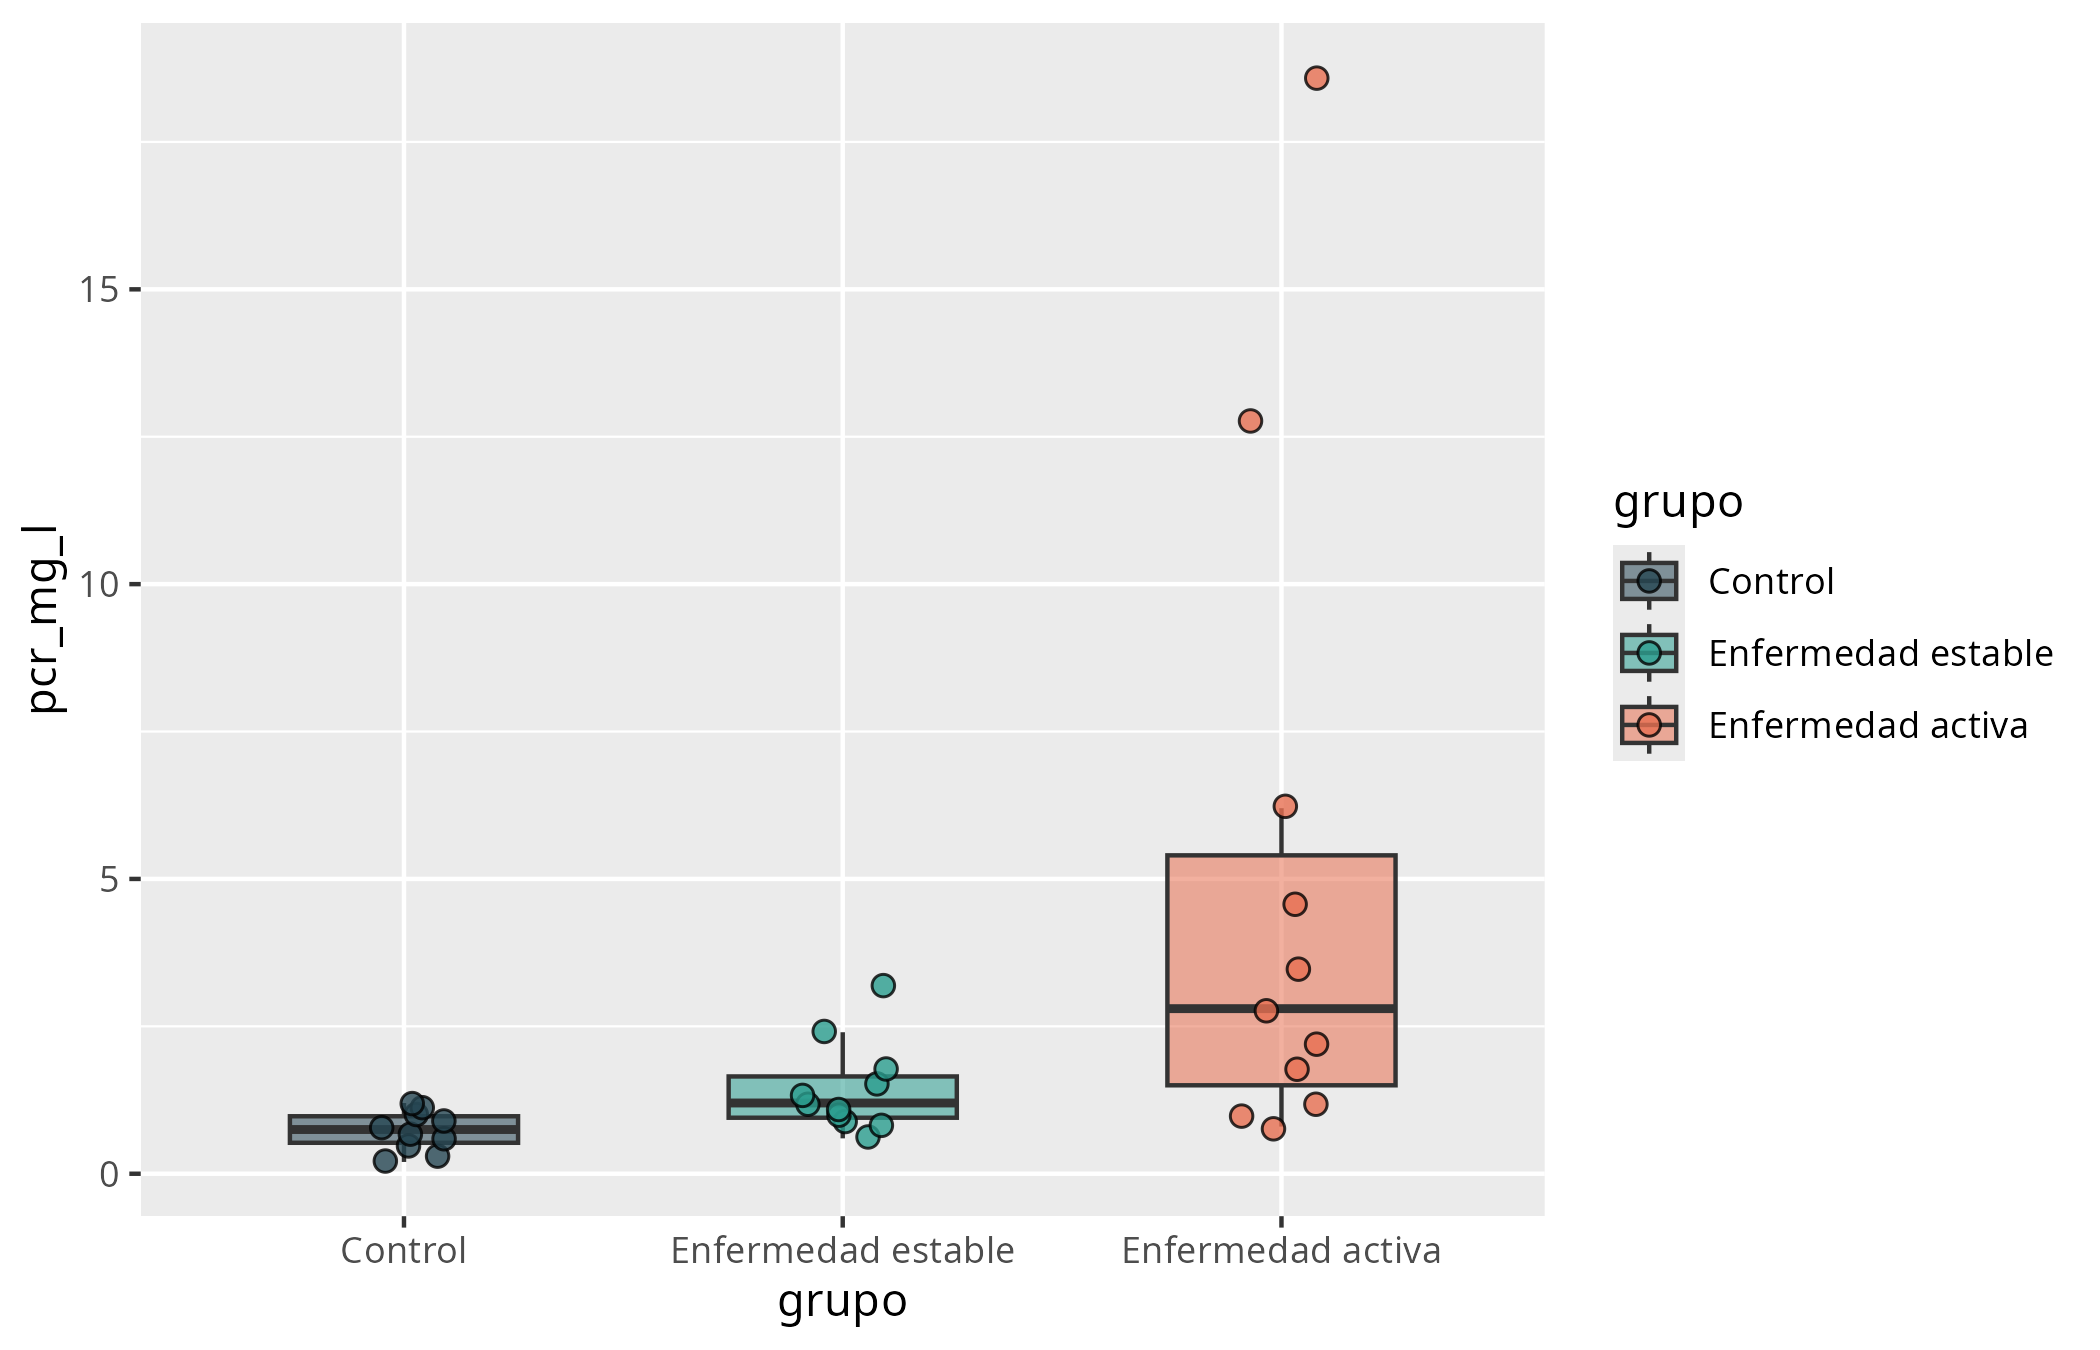
\includegraphics[width=\linewidth]{paso_3_colores.png}
\end{columns}
\end{frame}

% Lámina 6
\begin{frame}[fragile]{Paso 4. Etiquetas y tema de publicación}
\begin{columns}[T,onlytextwidth]
  \column{0.48\textwidth}
\begin{lstlisting}[basicstyle=\ttfamily\scriptsize]
grafico_publicacion <- paso_3 +
  geom_text(
    data = n_grupos,
    aes(grupo, 19.5,
        label = etiqueta),
    inherit.aes = FALSE
  ) +
  labs(
    x = NULL,
    y = "Proteína C reactiva (mg/L)"
  ) +
  coord_cartesian(ylim = c(0, 20)) +
  theme_classic(base_size = 12) +
  theme(legend.position = "none")
\end{lstlisting}
  \column{0.50\textwidth}
  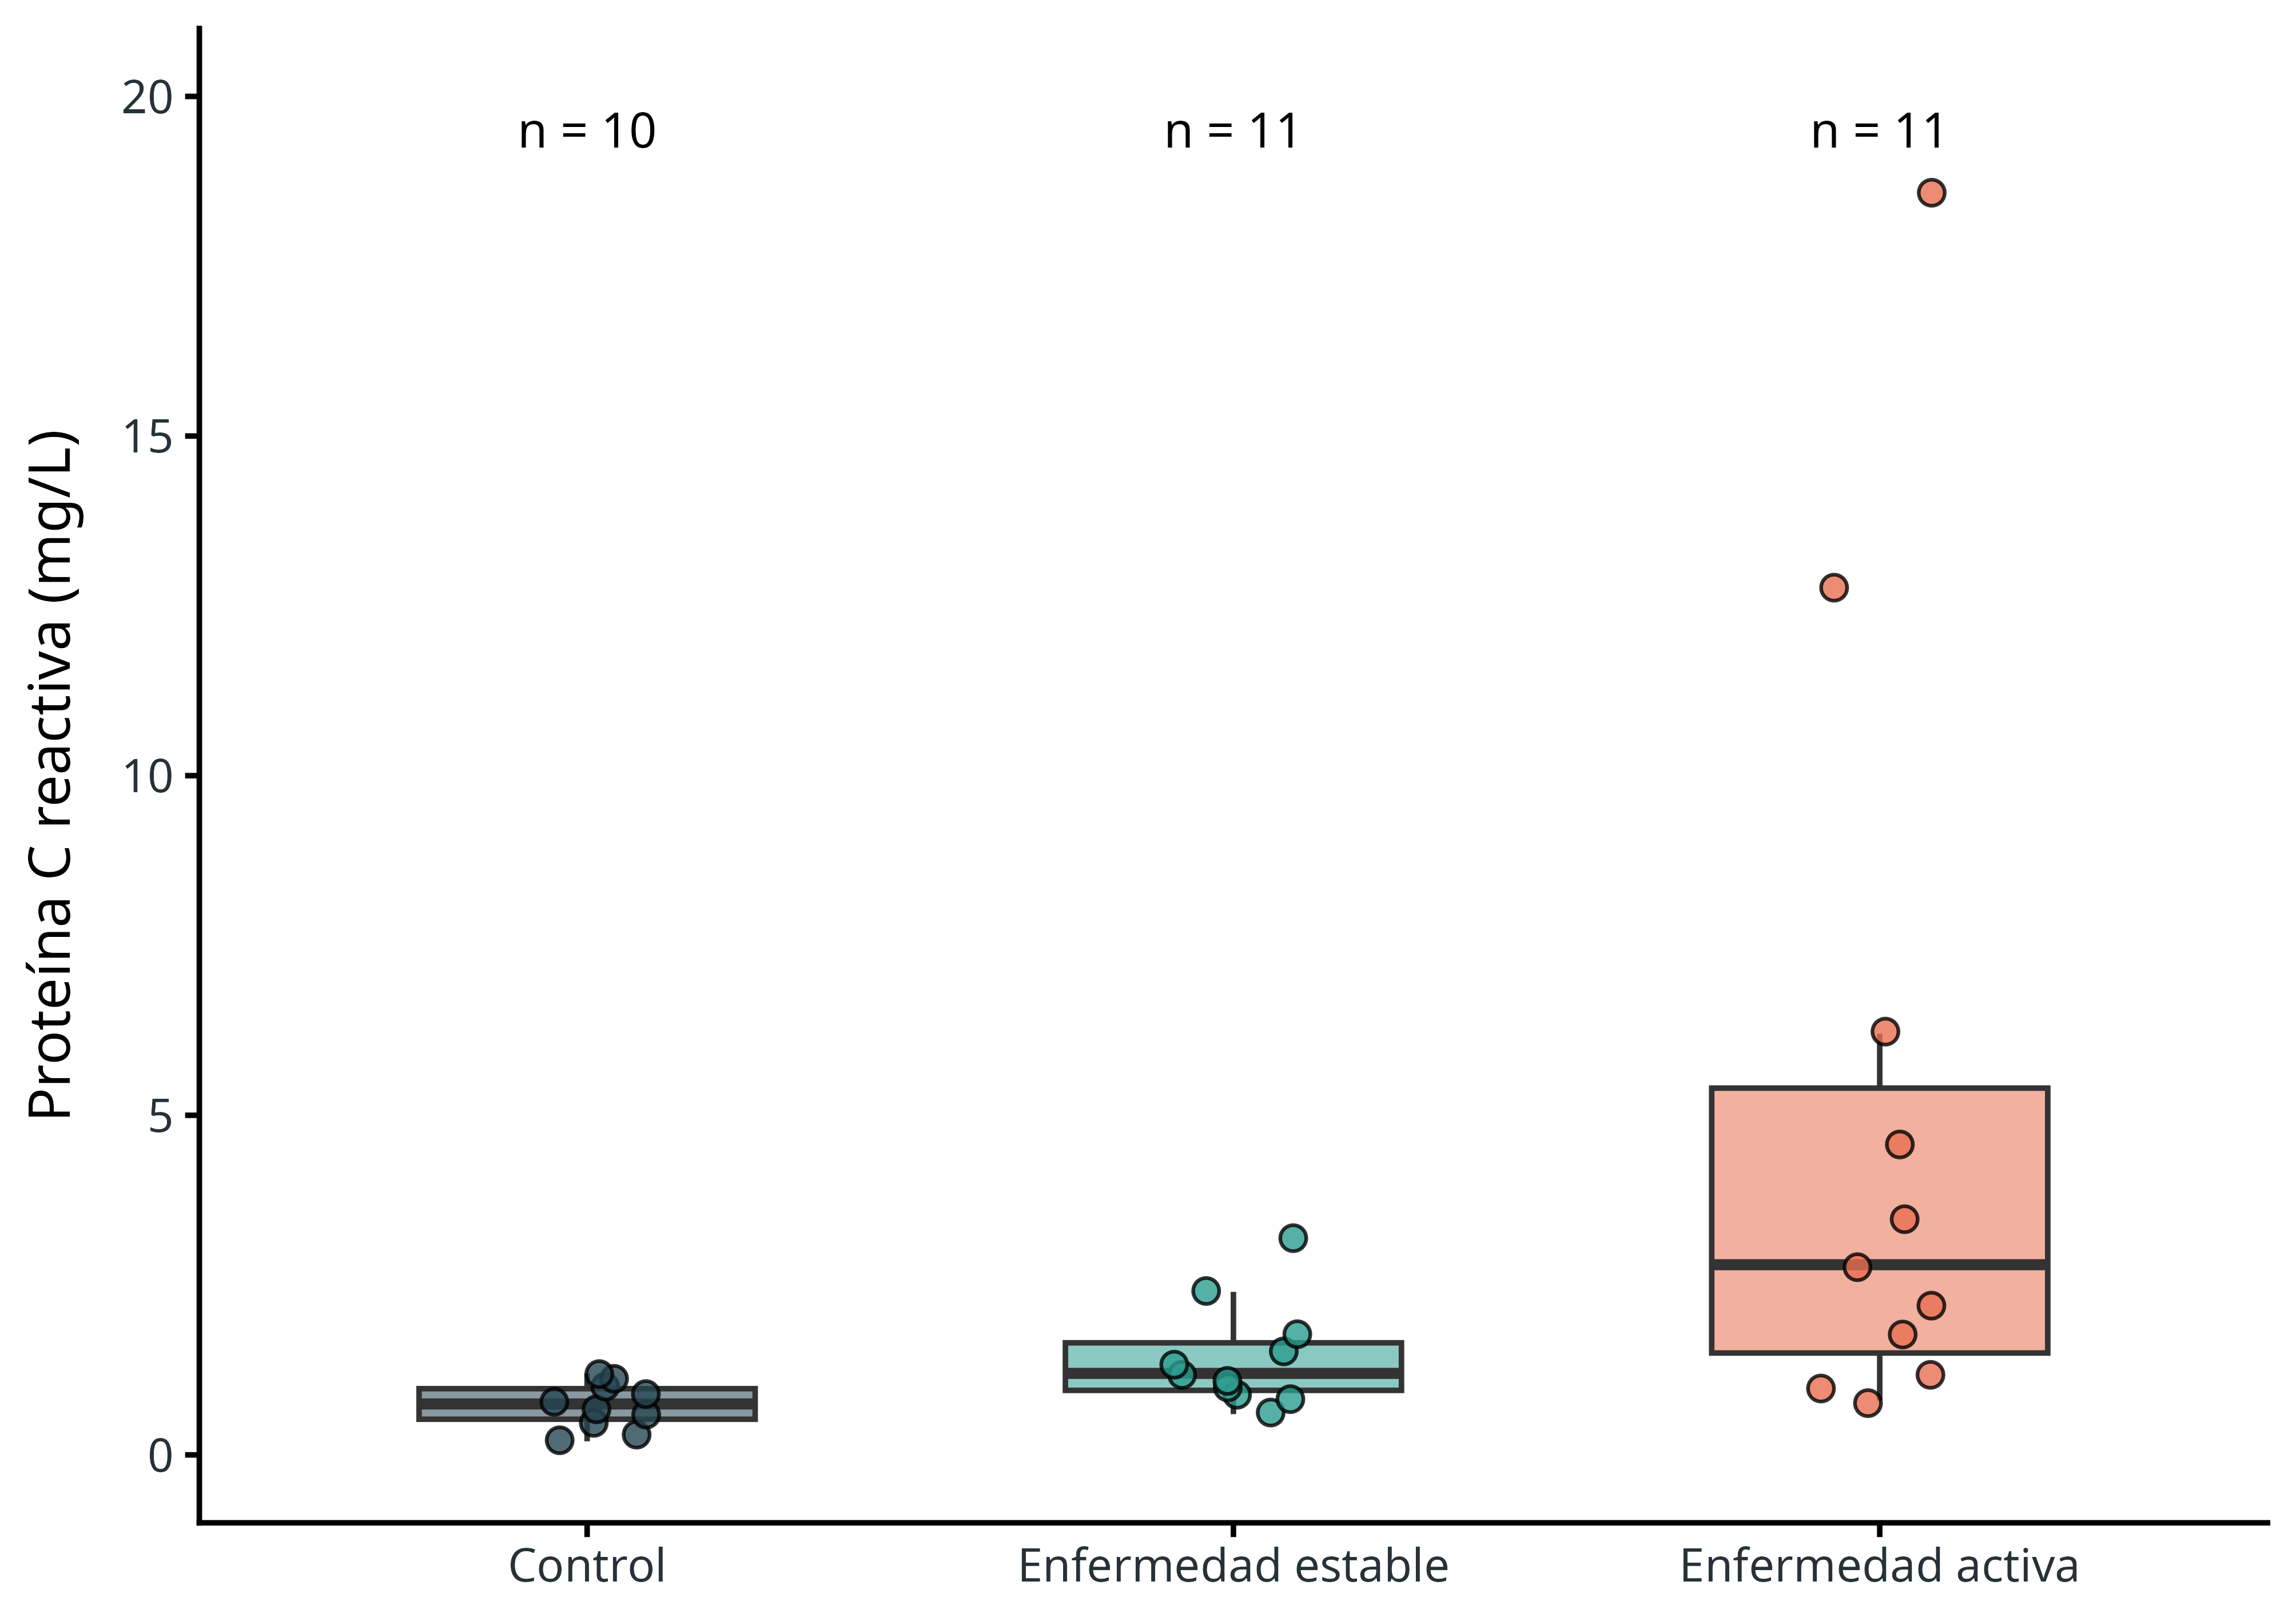
\includegraphics[width=\linewidth]{pcr_cajas_publicacion.png}
\end{columns}

\vspace{0.1cm}
\small Las unidades aparecen en el eje, el tamaño muestral queda visible y la leyenda desaparece porque los grupos ya están identificados.
\end{frame}

% Lámina 7
\begin{frame}[fragile]{Exportación y revisión final}
\begin{columns}[T,onlytextwidth]
  \column{0.49\textwidth}
\begin{lstlisting}[basicstyle=\ttfamily\scriptsize]
ggsave(
  "pcr_cajas_publicacion.png",
  grafico_publicacion,
  width = 170,
  height = 120,
  units = "mm",
  dpi = 600,
  bg = "white"
)
\end{lstlisting}

\small
El tamaño físico se define en milímetros. La resolución se ajusta a 600 dpi. La revista puede solicitar TIFF, PDF u otras dimensiones.
  \column{0.47\textwidth}
  \textcolor{verde}{\Large\textbf{Lista de comprobación}}\\[0.3cm]
  \begin{itemize}
    \item Variables y unidades correctas.
    \item Datos individuales visibles.
    \item Mediana y RIQ representados.
    \item Tamaño muestral informado.
    \item Colores distinguibles y consistentes.
    \item Texto legible al tamaño final.
    \item Formato conforme a la revista.
  \end{itemize}
\end{columns}

\vspace{0.10cm}
\centering
\textcolor{azul}{\small La figura describe los datos. Una comparación inferencial requiere otra prueba y su reporte correspondiente.}
\end{frame}

\end{document}
